\documentclass[aps,prb,reprint,amsfonts,amsmath,amssymb,showpacs,groupedaddress,superscriptaddress]{revtex4-1}
\usepackage{IEEEtrantools}
\usepackage{graphicx}
\usepackage{bm}
\usepackage{color}
% \usepackage{changes}
    % \definechangesauthor[name={Wang Shi}, color=orange]{swang}

\usepackage[colorlinks,urlcolor=blue,linkcolor=blue,anchorcolor=blue,citecolor=blue,bookmarks]{hyperref}

\begin{document}

\title{Global phase diagram and possible quantum spin liquid in the triangular $J-K-\Gamma$ model}

\author{Shi Wang}
\affiliation{National Laboratory of Solid State Microstructures and School of Physics, Nanjing University, Nanjing 210093, China}

\author{\textcolor{cyan}{XXX}}
\affiliation{\textcolor{cyan}{XXX}}
\author{\textcolor{cyan}{XXX}}
\affiliation{\textcolor{cyan}{XXX}}

\author{Shun-Li Yu}
\email{slyu@nju.edu.cn}
\affiliation{National Laboratory of Solid State Microstructures and School of Physics, Nanjing University, Nanjing 210093, China}
\affiliation{Collaborative Innovation Center of Advanced Microstructures, Nanjing University, Nanjing 210093, China}
\author{Jian-Xin Li}
\email{jxli@nju.edu.cn}
\affiliation{National Laboratory of Solid State Microstructures and School of Physics, Nanjing University, Nanjing 210093, China}
\affiliation{Collaborative Innovation Center of Advanced Microstructures, Nanjing University, Nanjing 210093, China}

\date{\today}

\begin{abstract}
\textcolor{red}{The global ground state phase diagram of the Heisenberg-Kitaev-$\Gamma$ model on a triangular lattice is studied using classical Monte Carlo and exact diagonalization. $\cdots \cdots$}
\end{abstract}

\maketitle

\section{Introduction}
Geometric frustration, which arises when the lattice geometry gives rise to constraints that cannot be simultaneously satisfied, plays an important role in various kinds of magnetic systems. In particluar, antiferromagnets on the triangular lattice are typical examples of such geometric frustated spin systems and have attracted numerous interests in condensed matter physics. For nearest-neighbor (NN) spin-$1/2$ antiferromagetic Heisenberg model on triangular lattice, though a fully disordered resonating-valence-bond (RVB) \cite{Anderson1973} state was proposed as the possible ground state in the early years, several studies point to a 120$^\circ$ N\'{e}el-ordered ground state thereafter \cite{PhysRevLett.99.127004,PhysRevLett.82.3899,PhysRevB.50.10048,PhysRevLett.60.2531}. When the second NN interactions are included which introduce further frustration, the system has a much richer phase diagram including a N\'{e}el phase, a phase with spin-wave selection of nontrivial ground states and a phase with incommensurate long-range order \cite{PhysRevB.42.4800,PhysRevB.46.11137}. All these studies have revealed that geometric frustated systems show quite different behavior from that of the non-frustated system.

On the other hand, exchange frustation in systems with strongly anisotropic magnetic interactions has been shown to be another promising approach to explore exotic quantum spin states. Like geometric frustation, the effect of exchange frustration is to prevent the formation of long range magnetic order and given raise to a residual ground-state entropy. The spin-$1/2$ Kitaev model \cite{Kitaev2006} on honeycomb lattice, which has both gapped and gapless quantum spin liquid (QSL) ground state (GS) supporting fractionalized excitations, is an example of a model with exchange frustration. As pointed out by Jackeli and Khaliullin \cite{Khaliullin2005, PhysRevLett.102.017205}, the elementary ingredients for realizing this highly anisotropic spin model are strong relativistic spin-orbit coupling (SOC), electron interactions, and specific geometric structure: edge sharing octahedra with 90$^\circ$ TM-O-TM bond angles. Because of its theoretical importance and potential application in quantum computing, great efforts have been made to search a solid-state realization of the Kitaev model. It was first proposed to be realized in iridates $A_2$IrO$_3$ (A = Na or Li) \cite{PhysRevLett.105.027204,PhysRevLett.108.127204,Chun2015,PhysRevLett.110.076402,PhysRevB.87.220407,PhysRevLett.110.097204,PhysRevLett.108.127203,PhysRevB.92.024413,PhysRevLett.112.077204,Rau2014}, and then turned towards $\alpha$-RuCl$_3$ \cite{PhysRevB.91.180401,Banerjee2016,PhysRevB.92.235119,PhysRevB.94.161106,PhysRevB.93.214431,PhysRevLett.118.107203,PhysRevLett.118.107203,PhysRevB.96.115103} in which Ir$^{4+}$/Ru$^{3+}$ ions are arranged in a honeycomb lattice and carry effective $j_{eff}=1/2$ moments. In fact, magnetic ions located at the center of edge-shared octahedra can not only form honeycomb lattice, but also triangular lattice (see Fig. \ref{fig:ModelDefinition}(a))and the Kitaev term can naturally be generalized to this scenario \cite{PhysRevB.93.104417,PhysRevB.89.014414}. Moreover, the symmetric off-diagonal $\Gamma$ term is allowed by symmetry and is a generic feature of S=$1/2$ models with edge sharing octahedra \cite {PhysRevLett.112.077204}. Kai Li \emph{et al.,} \cite{KaiLi2015} have studied the Heisenberg-Kitaev (HK) model on triangular lattice and a global phase diagram with a mean-field level chiral spin liquid (SL) as well as four magnetically ordered phases has been obtained. However, the effect of the $\Gamma$ term on triangluar lattice has not gain as much attention as on honeycomb lattice \cite{PhysRevLett.112.077204,Rau2014,PhysRevLett.118.107203,PhysRevB.96.115103,PhysRevB.93.214431,PhysRevB.100.144422}.

On the experimental side, the discovery of YbMgGaO$_4$ has invoked increasing interest in searching for rare-earth based spin-frustrated materials \cite{srep16419,PhysRevLett.115.167203,PhysRevB.94.035107,PhysRevB.96.054445,PhysRevB.97.184413,PhysRevB.97.125105,PhysRevB.96.075105,PhysRevLett.119.157201}. The Yb$^{3+}$ ions form a triangular layer and are surrounded by O$^{2-}$ which construct edge sharing octahedra \cite{srep16419,PhysRevLett.115.167203}. Extensive studies of magnetic properties using neutron scattering \cite{Nature20614,nphys3971,PhysRevLett.117.267202,PhysRevX.8.031001}, muon spin relaxation ($\mu$SR) \cite{PhysRevLett.117.097201}, electron spin resonance (ESR) \cite{PhysRevLett.115.167203} reveal a possible gapless quantum spin liquid (QSL) ground state. More recently, a class of compounds \emph{AReCh}$_2$ (A=alkali, Re=rare-earth, Ch=O, S, Se) with perfect triangular lattices of rare-earth ions have been synthesized and explored. The magnetic susceptibilty and heat capacity data suggest no long-range magnetic order or spin freezing down to the lowest measurement temperature, which implies their candidacy for QSL state \cite{acsmaterialslett.9b00464,PhysRevMaterials.3.114413,arXiv1911.08036,Liu_2018,arXiv1911.12712}. The novel magnetic properties of these triangluar magnets may be attributed to the interplay of geometric frustation and exchange frustration induces by spin-orbit coupling.

Inspired by previous theoretical and experimental works, we study the Heisenberg-Kitaev-$\Gamma$ ($J-K-\Gamma$) model on the triangular lattice. The $J-K-\Gamma$ model Hamiltonian is given by
\begin{equation}
    H=\sum_{\langle i,j \rangle \in \alpha \beta (\gamma)} \lbrack J \bm{S}_i \bm{\cdot} \bm{S}_j + K S_i^{\gamma} S_j^{\gamma} + \Gamma (S_i^{\alpha} S_j^{\beta} + S_i^{\beta} S_j^{\alpha}) \rbrack
    \label{eq:Hamiltonian}
\end{equation}
where $\langle i,j \rangle$ denotes the NN bonds, $\gamma$ takes value $x$, $y$, or $z$ depending on the direction of the NN bond as shown in Fig.\ref{fig:ModelDefinition}(b), and $\alpha$, $\beta$ are the remaining directions. $J$ and $K$ are the magnitude of the Heisenberg and Kitaev interactions and $\Gamma$ the symmetric off-diagonal exchanges. To the best of our knowledge, no exact solution has been reported so far for the spin-$1/2$ Kitaev and/or $\Gamma$ model on the triangular lattice. Therefore, it remains conceptually interesting to investigate whether the QSL could exist as a possible ground state of the triangular $J-K-\Gamma$ model.

\begin{figure}
    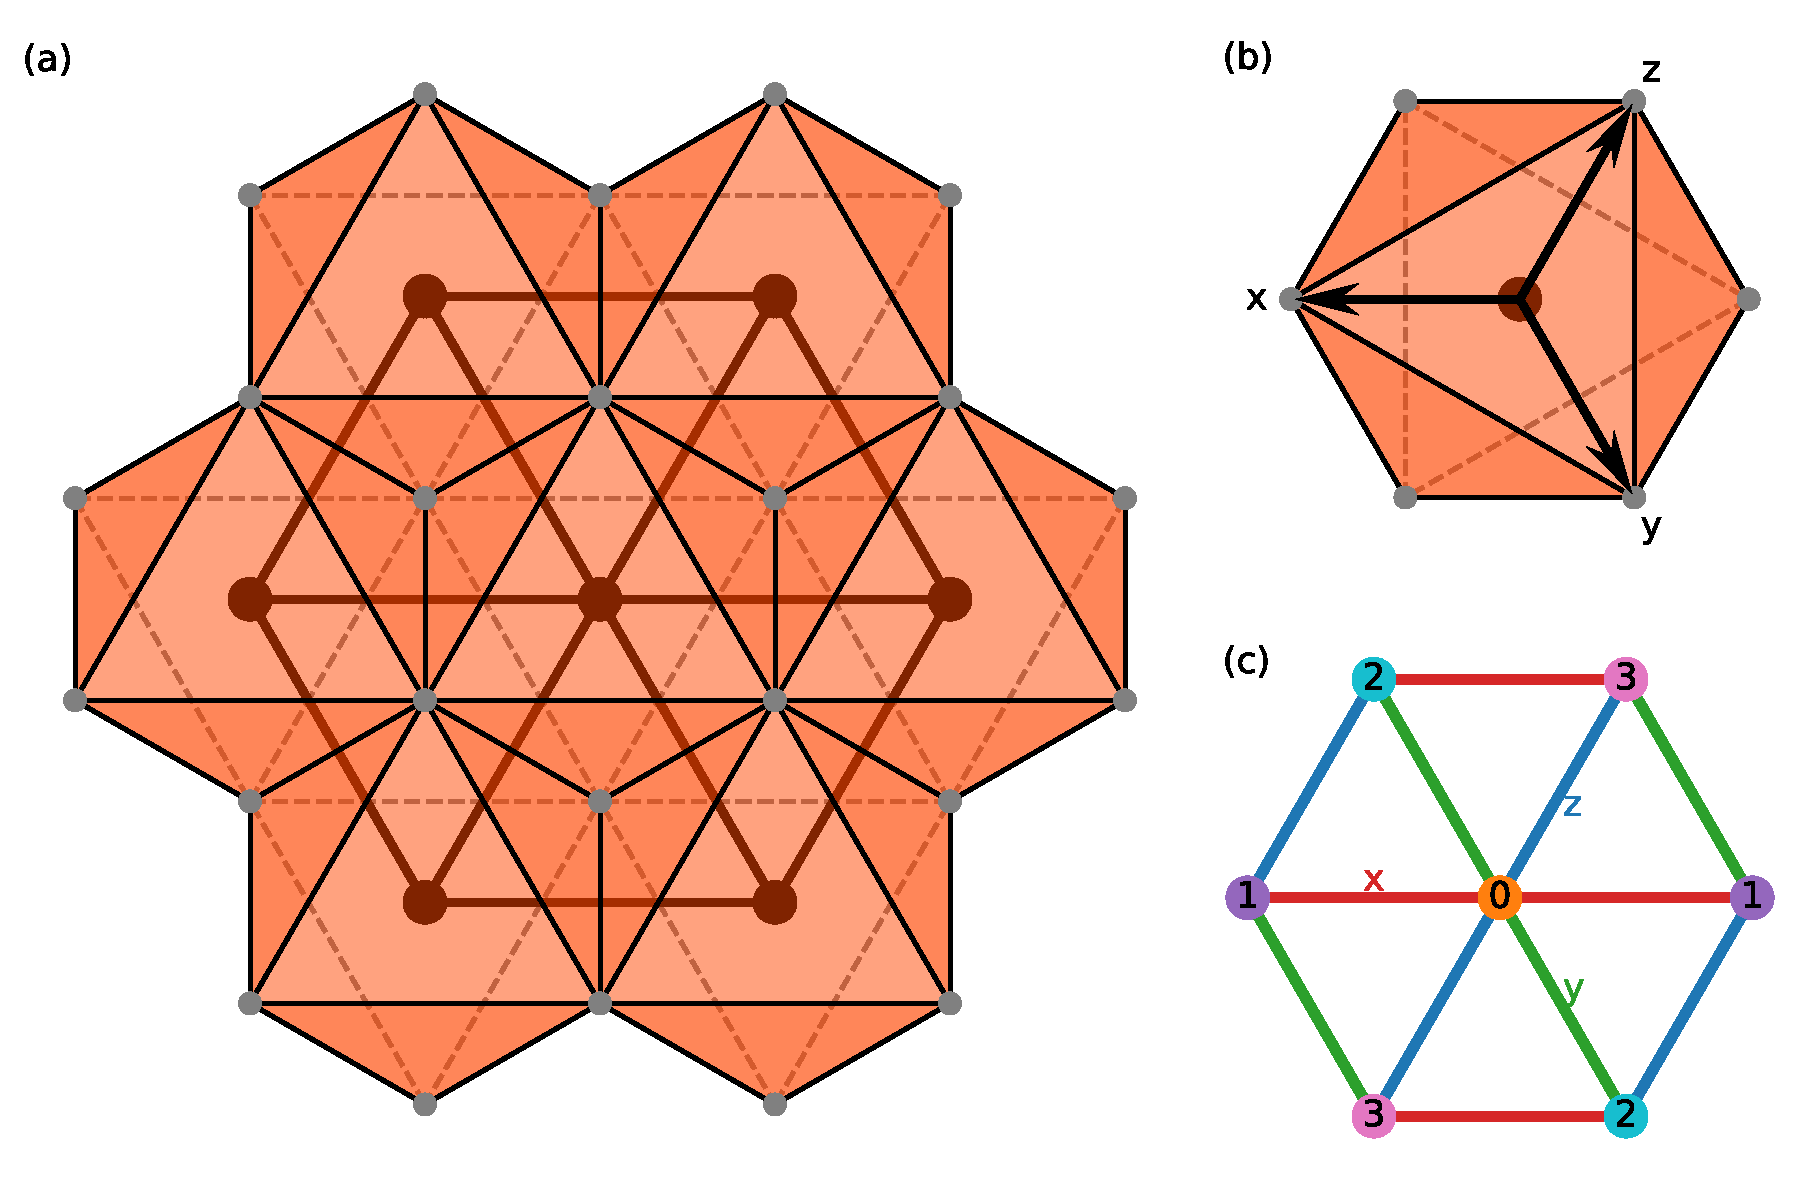
\includegraphics[width=\columnwidth]{Fig1.pdf}
    \caption{(Color online) (a) Top view of the triangular lattice of the edge-sharing octahedron. (b) Three types of the NN bonds on the triangular lattice, namely $\gamma=x, y, z$ colored red, green and blue, respectively. The different colors of the lattice sites label the four sublattices realizing the four-sublattice-transformation. (c) The orientation of the cubic $x$, $y$, $z$ axes with respect to the octahedron. The spin operators $S^x$, $S^y$ and $S^z$ are defined with respect to this reference frame.}
    \label{fig:ModelDefinition}
\end{figure}

The rest of the paper is organized as follows: The classical Monte Carlo and exact diagnoalization methods are introduced in Section II. Section III discusses the phases of the classical $J-K-\Gamma$ model with the main focus on the direction of the ordered moment of the FM and stripe states. The global phase diagram of the quantum model is presented in Section IV along with a discussion of its phases. In Section V, we study the moment direction of the quantum FM and stripe states, which provide characteristics to distinguish these phases.

\section{Methods}
The full anisotropic Hamiltonian \eqref{eq:Hamiltonian} is no longer exactly solvable, even for the classical case. One, therefore, either has to rely on approximate analytical method or on numerical techniques. To determine the ground state of the Hamiltonian \eqref{eq:Hamiltonian}, we employ a combination of classical Monte Cralo simulation and ED calculation. Here, we briefly describe the methods we used. For convenience, we fix the energy scale with $\sqrt{J^2 + K^2 + \Gamma^2}=1$ and parametrize the exchanges using angles $\alpha$ and $\beta$
\begin{equation}
    J=\sin\alpha \sin\beta, \quad K=\sin\alpha \cos\beta, \quad \Gamma=\cos\alpha
    \label{eq:Parameters}
\end{equation}
where $\alpha \in [0, \pi]$ and $\beta \in [0, 2\pi]$ to cover the global phase diagram.

\subsection{Classical Monte Carlo}
\textcolor{red}{A introduction to classical Monte Carlo.  To be accomplished $\cdots \cdots$}

\subsection{Exact Diagonalization}
We perform a Lanczos ED calculation of the GS energy of the Hamiltonian \eqref{eq:Hamiltonian} on several $4 \times 6$ clusters with periodic boundary conditions (PBC). To detect quantum phase transitions, the second derivatives of the ground-state energy, $-\partial^2E_0/\partial\alpha^2$ and $-\partial^2E_0/\partial\beta^2$ were computed and looked for singular features that indicate changes in the ground-state characteristics. Phases containing exactly solvable or well-understood points, such as the FM, 120$^\circ$ N\'{e}el, stripe and Dual N\'{e}el can be readily identified. The remaining phases were identified mainly by examining the static magnetic structure factor (SMSF)
\begin{equation}
    S(\mathbf{Q}) = \frac{1}{N} \sum_{ij}e^{i\mathbf{Q}\cdot(\mathbf{R}_i - \mathbf{R}_j)} \langle \mathbf{S}_i \cdot \mathbf{S}_j \rangle
    \label{eq:StaticStructureFactor}
\end{equation}
where N is the total number of spins, $\mathbf{R}_i$ is the position of site $i$ and $\langle \mathbf{S}_i \cdot \mathbf{S}_j \rangle$ is the average over the ground state.

To extract the moment direction of a magnetic ordered phase from a cluster ground state, we employ the method developed by Ji\v{r}\'{i} Chaloupka \emph{et  al} \cite{PhysRevB.94.064435}. The basic idea of this method is to measure the probabilities of the exact cluster GS on cluster spin-coherent states with varying moment directions. The cluster spin-coherent state is a direct product of spin-1/2 coherent states on each site $i$
\begin{equation}
    |\Psi\rangle = \bigotimes_{i=1}^N|\theta_i,\phi_i\rangle
    \label{eq:ClusterCoherentState}
\end{equation}
where the spin-1/2 coherent state
\begin{equation}
    |\theta, \phi \rangle = \mathcal{R}_z(\phi) \mathcal{R}_y(\theta) |\uparrow \rangle = e^{-i\phi S^z} e^{-i\theta S^y} |\uparrow\rangle
    \label{eq:Spin-1/2CoherentState}
\end{equation}
is fully polaried along the $(\theta, \phi)$ direction. Here the cubic axes are used (see Fig. \ref{fig:ModelDefinition}(c)), $\theta$ and $\phi$ are the conventional spherical angles, and $S^z |\uparrow \rangle = \frac{1}{2}|\uparrow \rangle$. By calculating the overlap with the exact cluster GS, and maximizing the probability $P = |\langle \Psi | GS \rangle|^2$ with respect to $\theta$s and $\phi$s, we can then identify the classical pattern that best fits the exact GS.

\section{Classical Analysis}
To understand the effects of inculding the off-diagonal $\Gamma$ term, we first study the classical $J-K-\Gamma$ model where the spin operators are viewed as unit-vectors in three dimension. On our proceeding, we note that the global phase diagram has been obtained previously by using a combination of Luttinger-Tsiza (LT) and classical Monte Carlo simulations \cite{PhysRevB.92.165108}. Six different magnetic orderings: ferromagnet (FM), stripe, 120$^\circ$ N\'{e}el order, nematic, $\mathbb{Z}_2$ and dual-$\mathbb{Z}_2$ vortex crystal phases were found, see Fig. 2 in Ref \onlinecite{PhysRevB.92.165108}. Our classical Monte Carlo study give qualitatively the same phase diagram.

\subsection{Moment direction of the classcial FM order}
For the classical FM order, the energy of the $J-K-\Gamma$ model per lattice site is given by
\begin{equation}
    E_{FM}^{c} = (3J + K) + 2\Gamma(S^xS^y + S^yS^z + S^zS^x)
    \label{eq:EcFM}
\end{equation}
where $S^x$, $S^y$, $S^z$ are the corresponding components of the classical moment vector. On this level, the moment direction of the classical FM state is determined solely by $\Gamma$ and the problem becomes finding the global minimum and maximum of the multi-variable function $f(S^x, S^y, S^z) = S^xS^y + S^yS^z + S^zS^x$ with the constraint $|\mathbf{S}| = 1$. $f(S^x, S^y, S^z)$ takes maximum value $f_{max}=1$ at $S^x=S^y=S^z=\pm 1/\sqrt{3}$ and minimum value $f_{min}=-0.5$ when the conditions $S^x + S^y + S^z = 0$ and $|\mathbf{S}| = 1$ are fulfilled. The condition $S^x + S^y + S^z = 0$ specify a plane that is perpendicular to the $[111]$ direction, and considering the reference frame shown in Fig. \ref{fig:ModelDefinition}(c) this is actually the plane of the triangular lattice. That is to say, for $\Gamma > 0$ the moment of the classcial FM state prefers to lie in the lattice plane and when $\Gamma$ is negative, the moment would perpendicular to the lattice plane.

Our classical Monte Carlo simulation found FM ordered state with the right moment direction for majority of the area marked as FM phase (see Fig. 2 in Ref \onlinecite{PhysRevB.92.165108}) except for the pure $\Gamma$ term. For pure positive $\Gamma$ interaction, apart from the FM order lie in the lattice plane, we also found disordered states which have the same energy as the FM state but no states with lower energy were found. When $\Gamma=-1$, in addition to the FM order perpendicular to the lattice plane, other long-range ordered states which are energetically degenerate with the FM state appear (see Appendix A for details). Based on these observation, it is reasonable to say that the ground state of the classical $\Gamma$ model is highly degenerate though the degeneracy may be lifted by introducing other interactions. For example, a ferromagnetic ($J<0$) Heisenberg interaction would break the degeneracy and select the FM order as the ground state which was verified by our Monte Carlo simulation. On the other hand, when positive Heisenberg interaction is included, which introduces further frustation to the system, the FM order is unlikely to be the GS. In fact, the classical GS were found to be disordered for $0 < J \ll \Gamma$ and stripe ordered for $0 < J \ll -\Gamma$. As for the disordered phase, when quantum flucations are involved, a quantum spin liquid state may emerge.

\subsection{Moment direction of the classcial stripe order}
In the case of stripe order, there are three degenerate spin configurations as illustrated in Fig. \ref{fig:PhaseDiagram}(b)-(d). For the spin configuration shown in Fig. \ref{fig:PhaseDiagram}(b), the energy of the model Hamiltonian \eqref{eq:Hamiltonian} is
\begin{IEEEeqnarray}{rCl}
    E_{StripeX}^{c} & = & -(J + K) + 2 K S^x S^x \nonumber \\
        && \negmedspace {} + 2 \Gamma (S^y S^z - S^z S^x - S^x S^y)
    \label{eq:EcStripeX}
\end{IEEEeqnarray}
and the energy for spin configuration in Fig. \ref{fig:PhaseDiagram}(c) and \ref{fig:PhaseDiagram}(d) can be obtained by a cyclic permutation $x \rightarrow y \rightarrow z \rightarrow x$. The moment direction of the classical stripe order is determined by the anisotropy parameters $K$ and $\Gamma$. In general ($J,K,\Gamma \neq 0$), $E_{StripeX}^{c}$ has three extreme points where the first derivatives equal zero
\begin{align}
    &\mathbf{S}_0: \quad S_{0}^{y}=-S_{0}^{z} = \pm1/\sqrt{2}, \quad S_{0}^{x} = 0 \label{eq:S0} \\
    &\mathbf{S}_1: \quad S_{1}^{y}=S_{1}^{z} = f_{1}(K, \Gamma), \quad S_{1}^{x} = g_{1}(K, \Gamma) S_{1}^{y} \label{eq:S1} \\
    &\mathbf{S}_2: \quad S_{2}^{y}=S_{2}^{z} = f_{2}(K, \Gamma), \quad S_{2}^{x} = g_{2}(K, \Gamma) S_{2}^{y} \label{eq:S2}
\end{align}
see Appendix B for their explicit expressions.

For $\Gamma=0, K>0$, it can be clearly seen from Eq\eqref{eq:EcStripeX} that the stripe order shown in Fig. \ref{fig:PhaseDiagram}(b) prefers to lie in the $yz$ plane. An infinitesimal positive $\Gamma$ would fix the ordered moment to the $\mathbf{S}_0$ direction whereas negative $\Gamma$ drives it to the $\mathbf{S}_1$ direction. When $\Gamma=0, K<0$, the moment would along the $x$-axis to have lowest energy, both positive and negative $\Gamma$ make it deviate from the $x$-axis and point to the $\mathbf{S}_1$ direction. All these stripe orders with the specific moment direction were found in the corresponding parameter space by our Monte Carlo simulation. However, in the HK limit ($\Gamma=0$), apart from the stripe orders lie in the axis plane, nematic orders which have the same energy were also found in the range $0 \leq |J| \ll K$.

\section{Global Phase Diagram}
\begin{figure*}
    \centering
    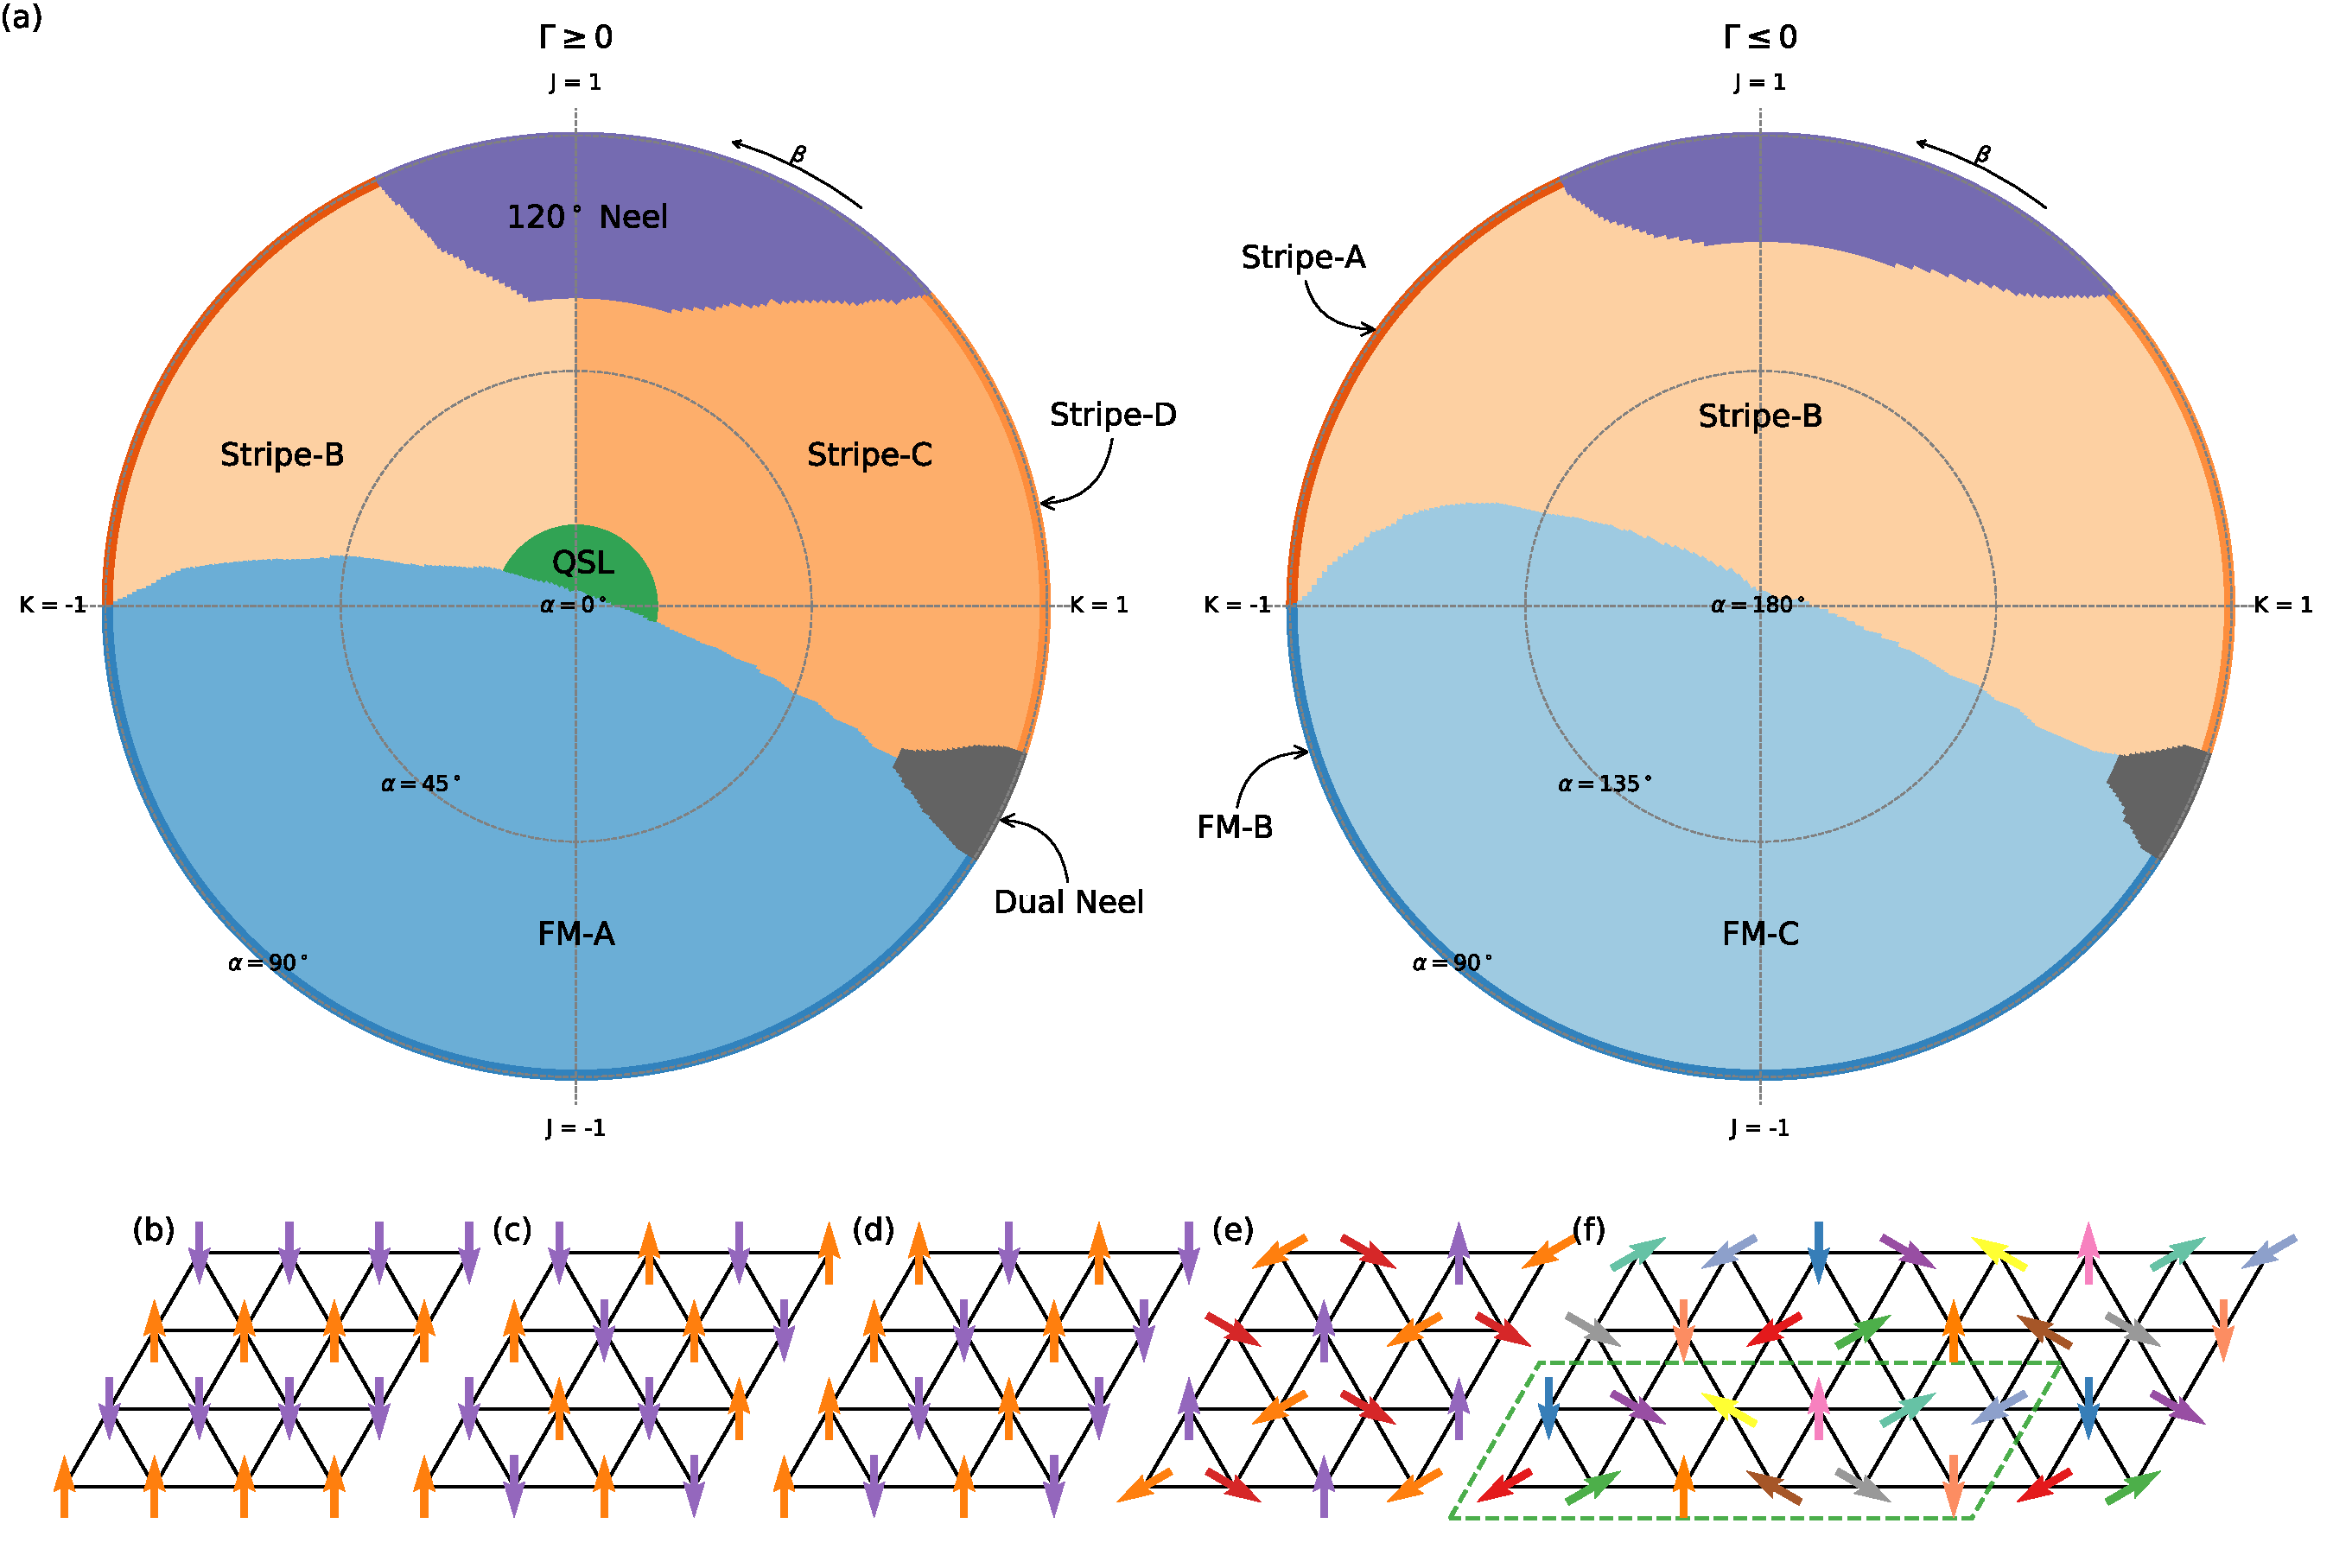
\includegraphics[width=0.96\textwidth]{Fig2.pdf}
    \caption{(Color online) (a) Global phase diagram of the triangular lattice J-K-$\Gamma$ model. The angle $\alpha$ and $\beta$ denote the radial and azimuthal angles, respectively. There are in total ten phases including three different FM phases denoted as FM-A, FM-B and FM-C, four different stripe phases designated as Stripe-A, Stripe-B, Stripe-C and Stripe-D, 120$^\circ$ N\'{e}el, Dual N\'{e}el and a possible quantum spin liquid phase. The three FM phases different from each other in the direction of the ordered moment, and also the four stripe phases are distinguished by their moment directions, see main text for details. (b)-(d) Illustation of the three degenerate spin configurations for all stripe orders. (e) Illustration of the 120$^\circ$ N\'{e}el order. All spins are coplanar and the angles between nearest-neighbor spins are 120$^\circ$. (f) Illustration of the Dual N\'{e}el order. The magnetic unit cell include 12 lattice sites as marked by the green dashed parallelogram.}
     \label{fig:PhaseDiagram}
\end{figure*}

In this section, we turn to study the quantum phases in the $J-K-\Gamma$ model Hamiltonian. We consider a $4 \times 6$ cluster with PBC that has been used previously to study the HK model on triangular lattice \cite{KaiLi2015}. The resulting phase diagrams for $\Gamma \geq 0$ and $\Gamma \leq 0$ are presented in Fig. \ref{fig:PhaseDiagram}(a). The phase boundaries are obtained from the location of singular features in $-\partial^2E_0/\partial\alpha^2$ and $-\partial^2E_0/\partial\beta^2$. The quantum phase diagram is closely resemble to the classical result in Ref. \onlinecite{PhysRevB.92.165108} except for the small green area near $\Gamma=1$ which does not appear in the classical phase diagram.

In the HK limit, by virtue of the existence of the so-called four-sublattice-transformation (FST) \cite{PhysRevB.89.014414}, two more magnetic ordered phases were identified in addition to the well-understood FM ($J=-1$)and 120$^\circ$ N\'{e}el ($J=1$) phases. Under the transformation, we obtain a collinear stripe order (see Fig. \ref{fig:PhaseDiagram}(b)-(d)) from the original FM order and a noncollinear spiral order (dual N\'{e}el) from the 120$^\circ$ N\'{e}el order (see Fig. \ref{fig:PhaseDiagram}(e) and (f)). The phase near the AF Kitaev point (i.e., $K=1$) has been proposed to be a chiral SL at the mean field level \cite{KaiLi2015} or a nematic phase in the quantum limit from DMRG calculation \cite{PhysRevB.91.155135}, however, a more recent study suggests that a stripe state is more likely to be the GS \cite{PhysRevX.9.021017}.

\begin{figure}
    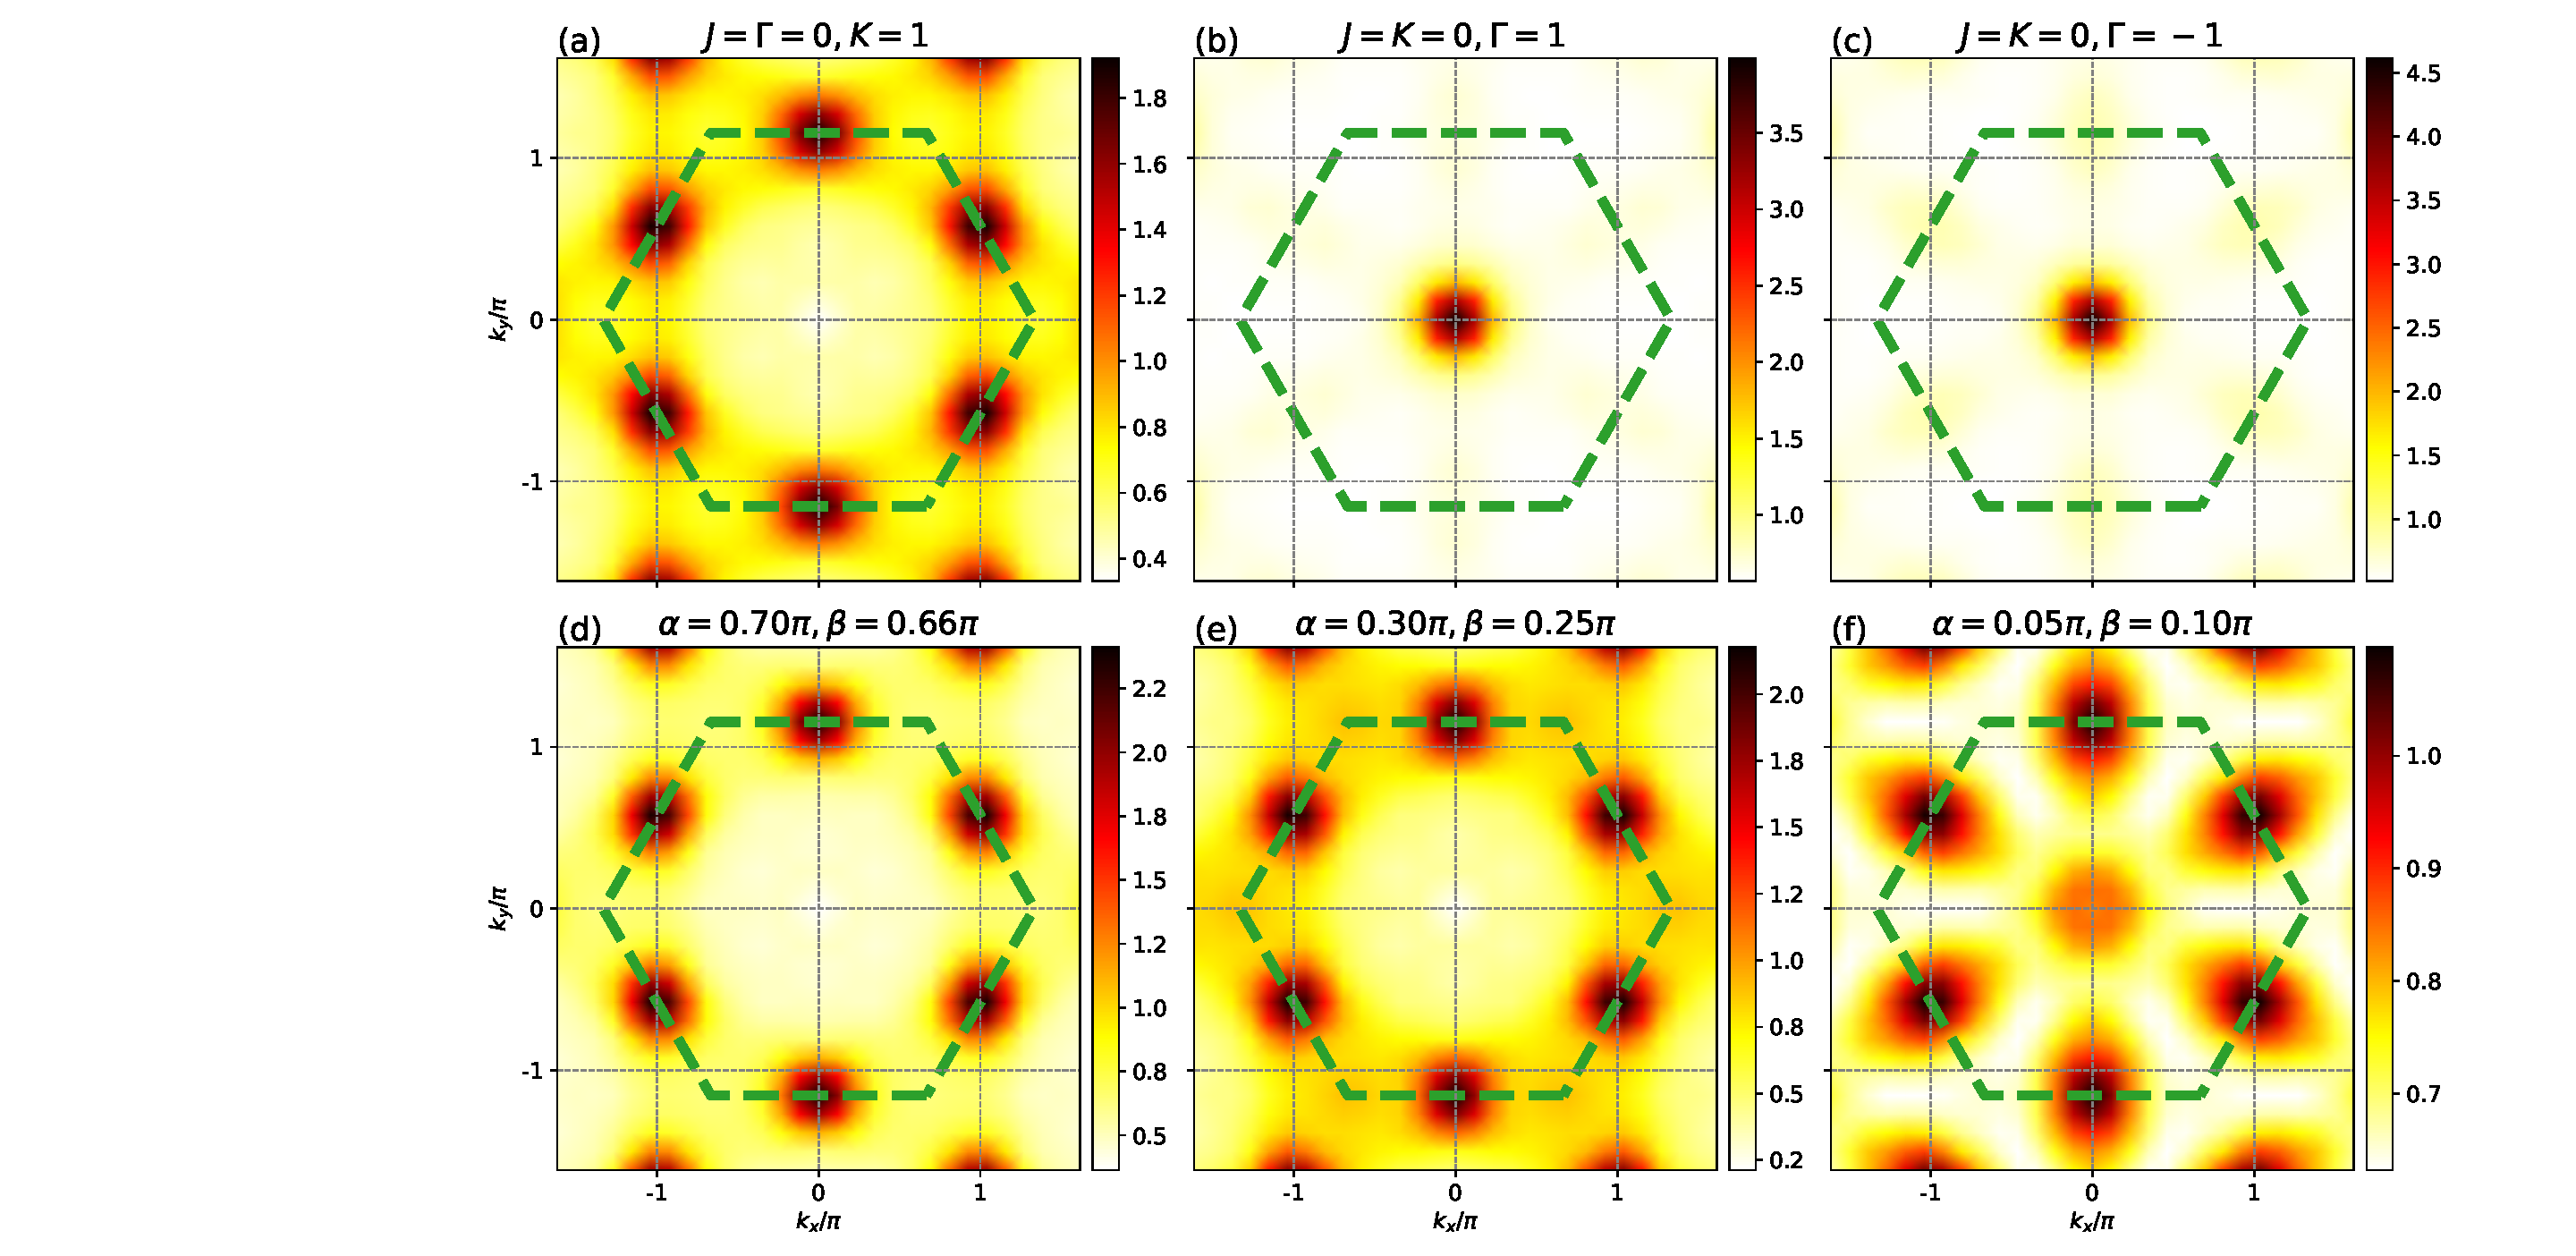
\includegraphics[width=0.45\textwidth]{Fig3.pdf}
    \caption{(Color online) SMSF for different model paramters. The green dashed lines marks the first BZ corresponding to the triangular lattice.}
     \label{fig:StructureFactors}
\end{figure}

When the off-diagonal $\Gamma$ term is included, the transforamtion is no longer valid. To identify the remaining phases and providing more information of these phases, we calculate the SMSF for some representative model paramters, as shown in Fig. \ref{fig:StructureFactors}. For pure $\Gamma$ model, see Fig. \ref{fig:StructureFactors}(a) and (b), the peak of the SMSF locates at the center of first Brillouin Zone (BZ) which is a typical characteristic of the FM order. Take into account of the classical results, we propose the three blue areas with different shadings in the global phase diagram (see Fig. \ref{fig:PhaseDiagram}) to be FM ordered phases (i.e., \emph{FM-A}, \emph{FM-B}, \emph{FM-C}) and they different from each other in the direction of the ordered moment which will be discussed in the next section. In Fig. \ref{fig:StructureFactors}(c)-(e), the SMSF peaked at the M-points indicating that the stripe ordered GS of the classical model persist in the quantum limit. It is worth to note that even the GS of the classical model near the AF Kitaev point was identified to be nematic ordered which is energetically degenerate with the stripe state, our ED results favor the idea that quantum flucations would select a stripe state. The four stripe phases designated as \emph{Stripe-A}, \emph{-B}, \emph{-C}, \emph{-D} in Fig. \ref{fig:PhaseDiagram}(a) different from each other only in the moment direction. Apart from these single-$\mathbf{Q}$ phases, we also identify a multi-$\mathbf{Q}$ phase, see the green area in Fig. \ref{fig:PhaseDiagram}(a). For $J$, $K$, $\Gamma$ in this area, the SMSF has high intensities at both the center and M-points of the first BZ and Fig. \ref{fig:StructureFactors}(f) is a typical SMSF profile of this phase. \textcolor{red}{$\cdots \cdots$}

\section{Moment Direction-Exact Diagonalization Results}
\begin{figure}
    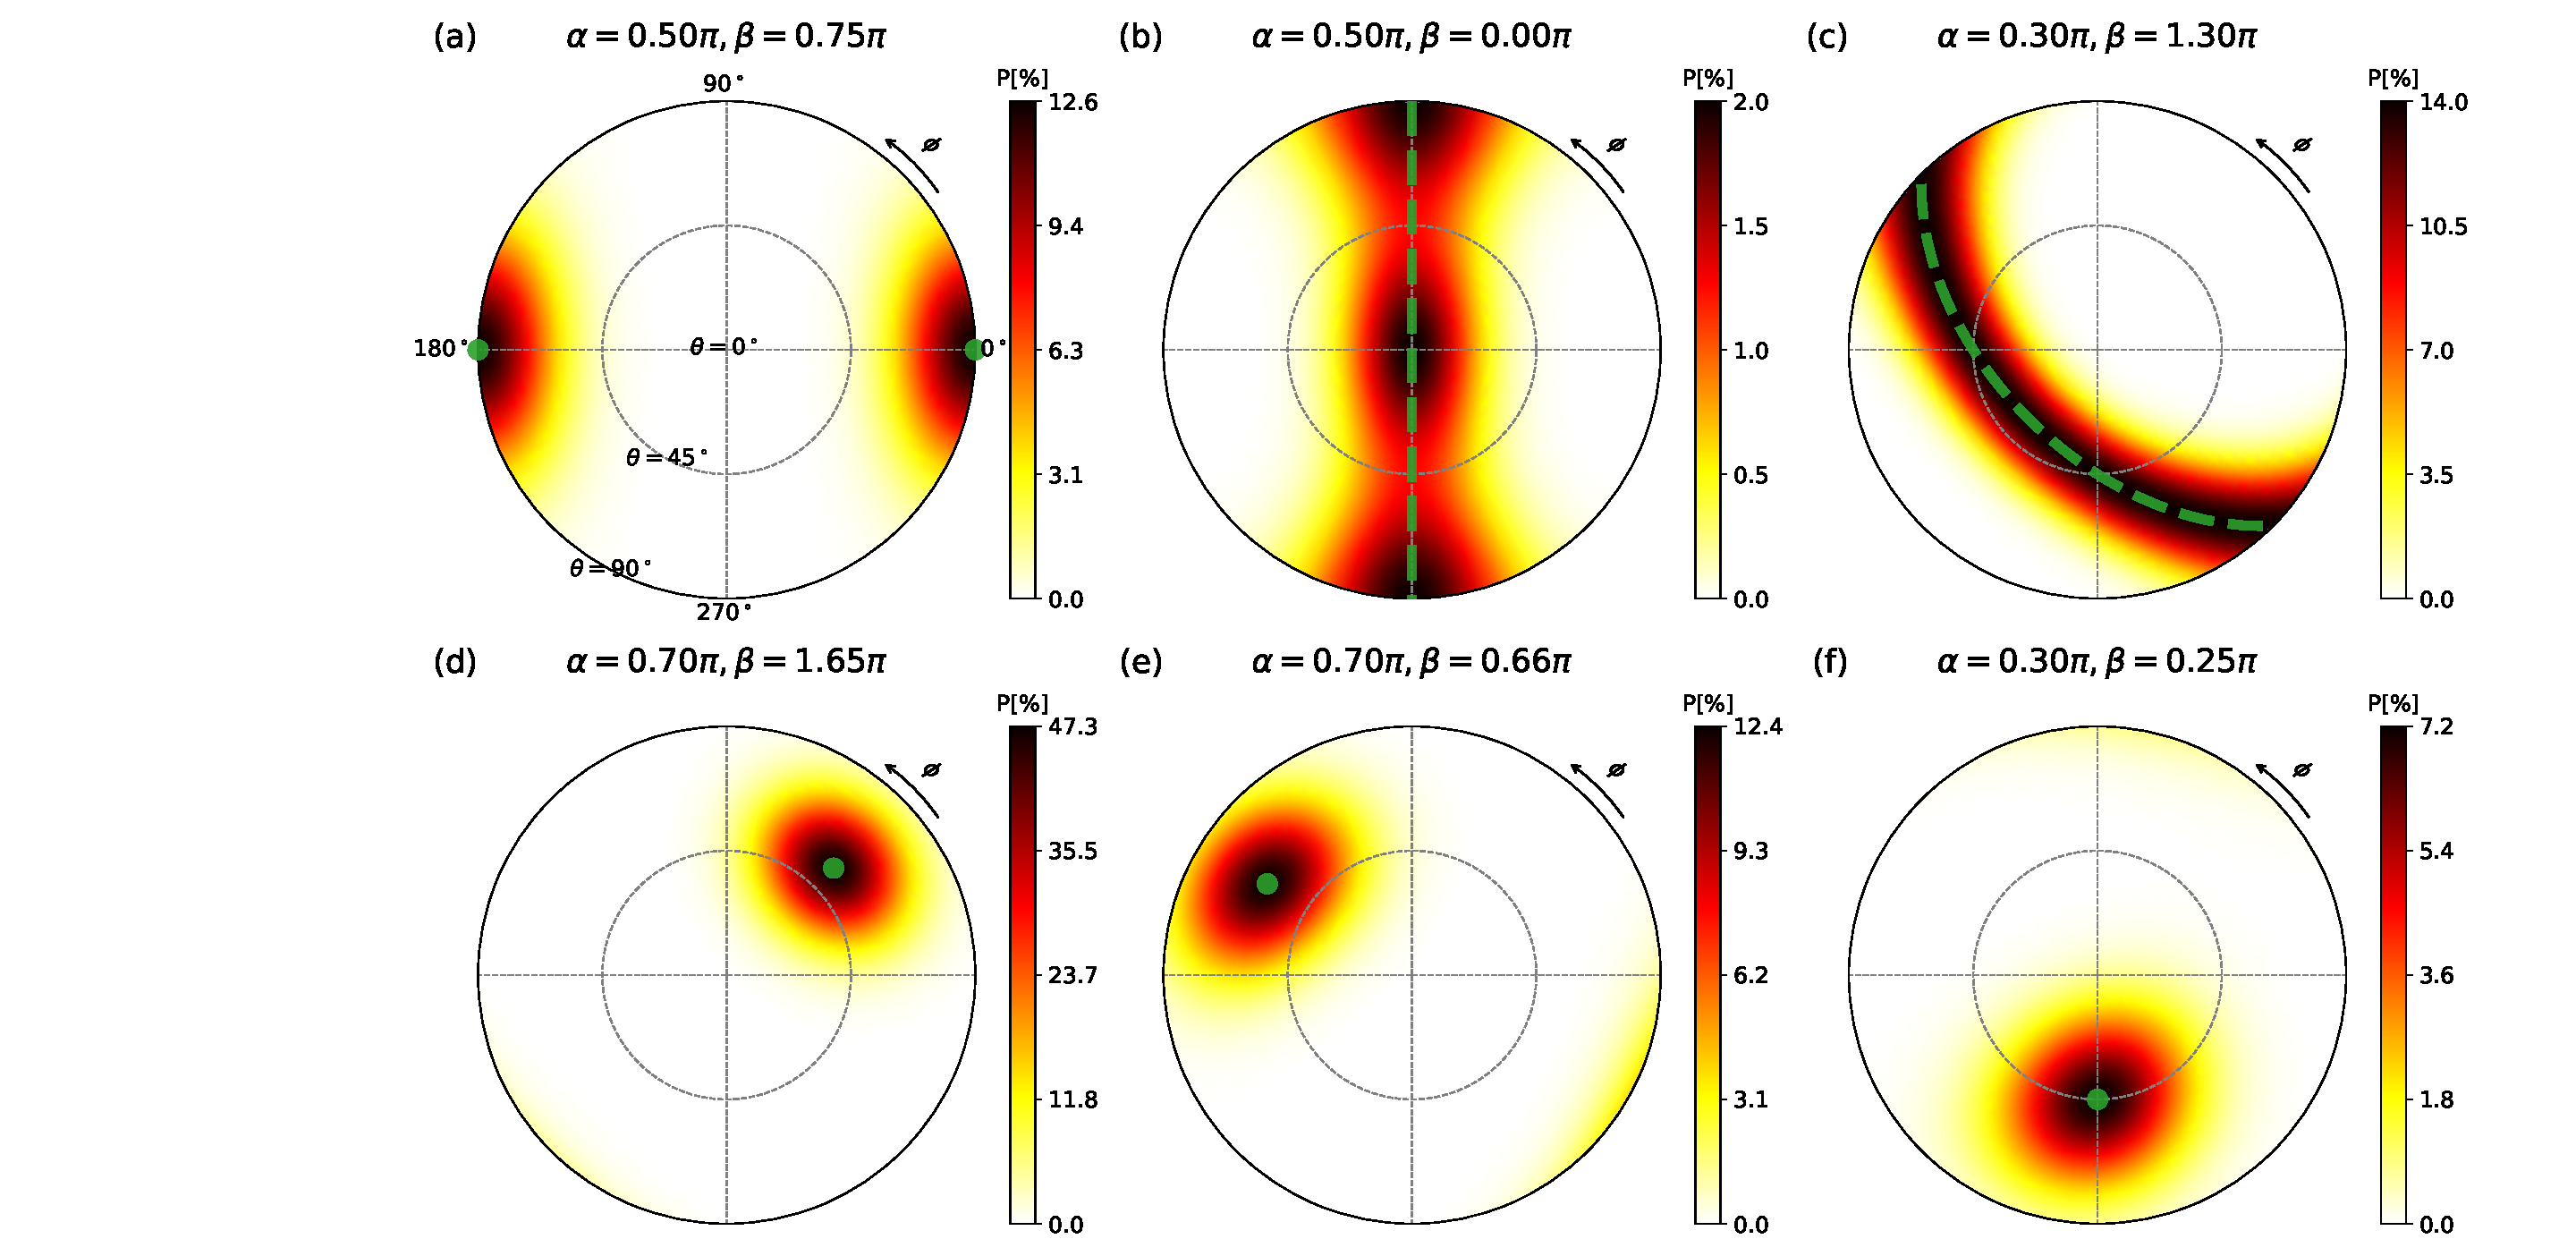
\includegraphics[width=0.45\textwidth]{Fig4.pdf}
    \caption{\label{fig:Proabilities}(Color online) Map of the probabilities of the cluster spin-coherent state given by Eq.\eqref{eq:ClusterCoherentState} in varies exact cluster GS. The radial and polar coordinate gives the angles $\theta$ and $\phi$, which are spherical angles with respect to the reference frame shown in Fig. \ref{fig:ModelDefinition}(c). The green dashed lines and solid circles mark the ordered moment direction for the classical states, see main text for details. (a)-(b) Probability maps for the FM states in the \emph{FM-A} and \emph{FM-C} phase, respectively. (c)-(f) Proability maps for the stripe states in the \emph{Stripe-A}, \emph{Stripe-B}, \emph{Stripe-C} and \emph{Stripe-D} phase, respectively.}
\end{figure}

Having map out the global phase diagram of the $J-K-\Gamma$ model, we now move to the moment direction of these FM and stripe phases which provides key characteristic to distinguish them. Since the cluster spin-coherent state is captured by only a single pair ($\theta$, $\phi$) for collinear phases (in our case, these are FM and stripe), it is easy to determine the direction of the ordered moment by inspecting the probability map $P(\theta, \phi) = | \langle \Psi (\theta, \phi) | GS \rangle |^2.$

\subsection{Moment direction of the FM phases}
For pure Heisenberg model, the FM state is spin rotational invariant and the ordered moment can point any direction. The easy axis Kitaev interaction breaks the accidental spin rotational symmetry, pinning the orderings to the axis direction(i.e., \textit{x}, \textit{y}, \textit{z} direction). However, when the off-diagonal $\Gamma$ term is introduced, which would compete with Kitaev interaction, the moment orientation will deviate from the axis direction. To extract the moment direction of the \emph{FM-A} and \emph{FM-C} phases, we construct the following cluster spin-coherent state
\begin{equation}
    |\Psi(\theta, \phi) \rangle = \bigotimes_{i=1}^N|\theta,\phi \rangle
\end{equation}
and calculate the probabilities $P(\theta, \phi)$ with varying $\theta$ and $\phi$. The resulting probability maps are shown in Fig. \ref{fig:Proabilities}(a) and \ref{fig:Proabilities}(b). For the \emph{FM-A} phase, the probability map reveals the moment being constrained to the lattice plane with all directions degenerate, as expected from classical considerations (see the green dashed line). As for the \emph{FM-C} phase, the probability is clearly peaked at the direction perpendicular to the lattice plane which is also consistent with our classical analysis (marked by the green solid circle).

\subsection{Moment direction of the stripe phases}
The stripe phases have three degenerate patterns as shown in Fig. \ref{fig:PhaseDiagram}(b)-(d) and the ordered moment is locked to the orientation of the stripe pattern. For brevity, we only construct cluster spin-coherent state based on the stripe pattern shown in Fig. \ref{fig:PhaseDiagram}(b) and present the probability maps in Fig. \ref{fig:Proabilities}(c)-(f) for \emph{Stripe-A}, \emph{Stripe-B}, \emph{Stripe-C}, \emph{Stripe-D} respectively. In the HK limit, the \emph{Stripe-A} phase is connected to the \emph{FM-B} phase through FST and the spins are supposed to along the \emph{x}-axis for stripe pattern in Fig. \ref{fig:PhaseDiagram}(b) from classical considerations, our ED results show that this situation also applies at quantum limit (see Fig. \ref{fig:Proabilities}(c)). As for the \emph{Stripe-D} phase near the AF Kitaev point, the probability map Fig. \ref{fig:Proabilities}(f) reveals the moment being constrained to the vicinity of the \emph{yz} plane, as predicted by classical analysis. Within this plane, the order-from-disorder mechanism selects the cubic axes \emph{y} and \emph{z} where the probability reaches its maxima. The small $P_{max}$ of about 3\% can be partly attributed to the cluster GS being a superposition of six possible classical stripe states, more importantly it a signature of large quantum flucations in the ground state.

The main effect of $\Gamma$ term on the \emph{Stripe-A} and \emph{Stripe-D} phase is tilting the moment orientation away from the cubic axes directions, yielding the \emph{Stripe-B} and \emph{Stripe-C} phase. Fig. \ref{fig:Proabilities}(e) is a representative probability map for the \emph{Stripe-B} phase. The probability takes maximum value at the direction determined by Eq.\eqref{eq:S1}, which means that the moment direction changes with the model parameters $K$ and $\Gamma$. On the other hand, the case of the \emph{Stripe-C} phase is rather different. The probability is clearly peaked at the direction given by Eq.\eqref{eq:S0} with the maximum value $P_{max}$ considerably less than $\frac{1}{6}$ (see Fig. \ref{fig:Proabilities}(d)). Apart from the overall reduction factor of $\frac{1}{6}$ due to the six possible stripe states being superposed in the cluster GS, quantum flucations may take responsibilities for the reduced probability.

\section{Summary}
\textcolor{red}{Summary of our work. To be accomplished $\cdots \cdots$}

\begin{acknowledgments}
    \textcolor{red}{Acknowledgements.  To be accomplished $\cdots \cdots$}
\end{acknowledgments}


% The following are the Appendixes of this article
\appendix

\section{Analysis of the classical energy and moment direction}

\textcolor{red}{Analysis of the classical energy and moment direction. To be accomplished $\cdots \cdots$}

\newpage

\bibliography{ref}

\end{document}
